\begin{surferPage}[חרוט כפול]{חרוט כפול}
   כפי שהסברנו במבוא לגלריית תמונות זו, משטח מכונה
    \emph{לא-סינגולרי} או חלק אם אינו כולל שום קדקוד
    (קדקודים כאלה מכונים נקודות סינגולריות).
    לדוגמה, ספֶרָה או טוֹרוּס (שתי התמונות השמאליות להלן):
    \begin{center}
      \begin{tabular}{@{}c@{}c@{}c@{}c@{}}
        \begin{tabular}{@{}c}
          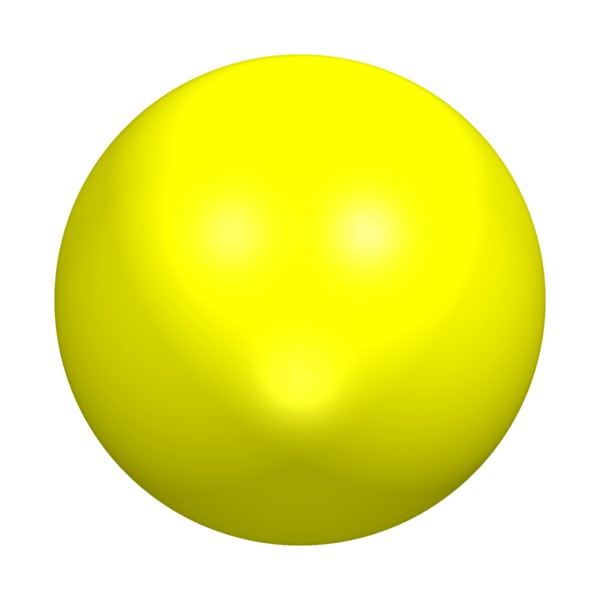
\includegraphics[width=1.4cm]{./../../common/images/kugel}
        \end{tabular}
        &
        \begin{tabular}{@{}c}
          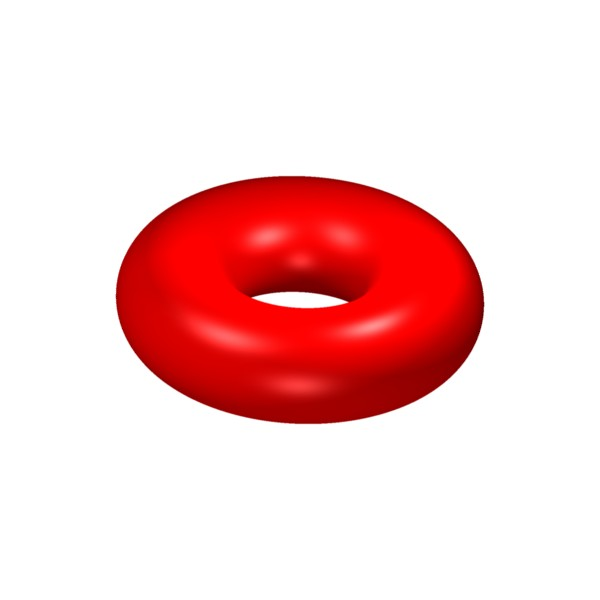
\includegraphics[width=1.4cm]{./../../common/images/torus}
        \end{tabular}
        &
        \begin{tabular}{c@{}}
          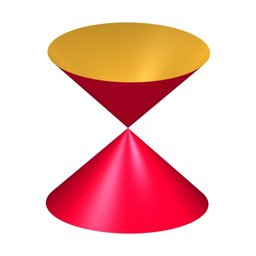
\includegraphics[width=1.4cm]{./../../common/images/kegel}
        \end{tabular}
      \end{tabular}
    \end{center}
     החרוט הכפול (התמונה הימנית) הוא הסינגולריות הפשוטה ביותר; זוהי הסינגולריות היחידה שניתן לתאר באמצעות משוואה
    ממעלה $2$:
    \[x^2+y^2-z^2=0.\]
    כאשר משנים מעט משוואה זו, על-ידי החלפה של ה-$0$ בערך קטן
    $a\neq 0$, החרוט הכפול הופך לאחד משני סוגי
    ההיפֶּרבּוֹלוֹאידים, בהתאם לסימן של $a$:
    \begin{center}
      \begin{tabular}{@{}c@{\ }c@{\ }c@{\ }c@{\ }c@{}}
        \begin{tabular}{@{}c@{}}
          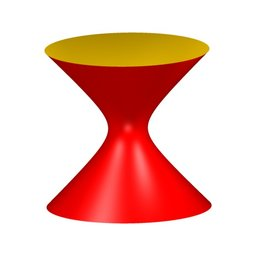
\includegraphics[width=1.2cm]{./../../common/images/A1pm_2}
        \end{tabular}
        &
        $\leftarrow$
        &
        \begin{tabular}{@{}c@{}}
          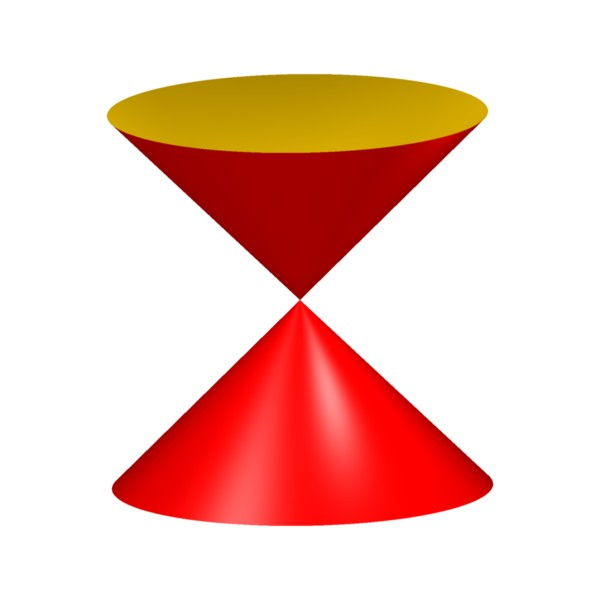
\includegraphics[width=1.2cm]{./../../common/images/A1pm_1} 
        \end{tabular}
        &
        $\rightarrow$
        &
        \begin{tabular}{@{}c@{}}
          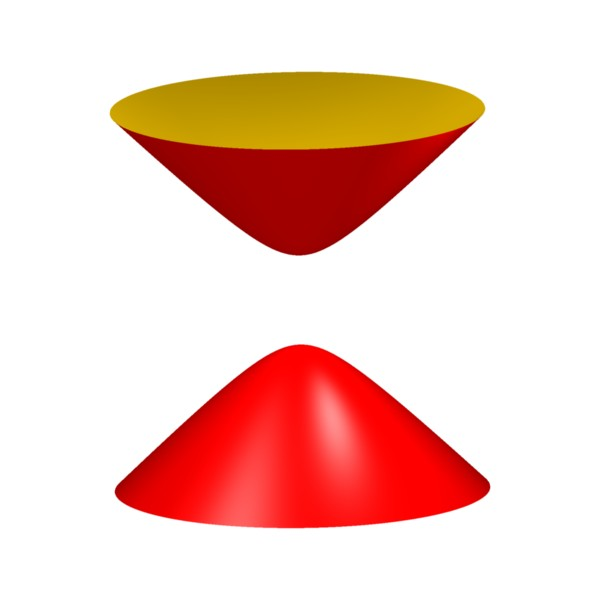
\includegraphics[width=1.2cm]{./../../common/images/A1pm_0}
        \end{tabular}
      \end{tabular}
    \end{center}
   במשטח ממעלה $2$ לא יכולה להיות יותר מנקודת סינגולריות אחת, כלומר $\mu(2)=1$.
\end{surferPage}
